\documentclass[12pt]{article}
\usepackage[utf8]{inputenc}
\usepackage[
a4paper,		% papel A4
left=2cm,		% margem esquerda
right=2cm,		% margem direita
top=2cm,		% margem superior
bottom=2cm		% margem inferior
]{geometry}
\usepackage[T1]{fontenc}	
\usepackage{array,latexsym}
\usepackage{amsmath,amsfonts,amssymb,amsthm,mathabx,amstext}
\usepackage{dsfont}	% Conjuntos: $\mathds{N, Z, Q, R, C}$
\usepackage{graphicx}
\begin{document}
\begin{center}
	Universidade Federal da Paraíba\\
	Probabilidade II - Primeira prova\\
	Paulo Ricardo Seganfredo Campana 
\end{center}

\noindent Questão 1.\\

\noindent a)\\
	
$F'(x)=f(x)$\\

$\dfrac{d}{dx}\left(0\right)=0$\\

$\dfrac{d}{dx}\left(-\dfrac{1}{2}(x^{2}-1)\right)=-x$\\

$\dfrac{d}{dx}\left(\dfrac{1}{2}(x^{2}+1)\right)=x$\\

$\dfrac{d}{dx}(1)=0$\\

$f(x)=\left\{\begin{array}{@{}l@{}}
	-x\text{, se }-1<x<0,\\
	x\text{,\quad se }0<x<1,\\
	0\text{,\quad caso contrário.}
\end{array}\right.$\\

\begin{figure}[h!]
	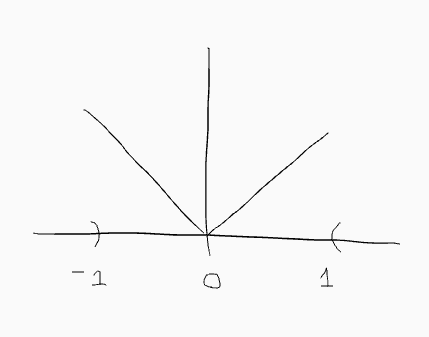
\includegraphics[scale=0.7]{q1}
\end{figure}

$S_{X} = [-1,1]$\\

\noindent b)\\

Os pontos -1 e 1, pois as derivadas laterais são diferentes.\\

Para $x=-1^{-}$ a derivada no ponto é 0

Para $x=-1^{+}$ a derivada no ponto é 1

Para $x=1^{-}$ a derivada no ponto é 1
 
Para $x=1^{+}$ a derivada no ponto é 0\\

\noindent c)\\

$P\left(-\dfrac{1}{2}<x<\dfrac{1}{2}\right)=P\left(-\dfrac{1}{2}<x<0\right)+P\left(0<x<\dfrac{1}{2}\right)$\\\\

$\displaystyle\int_{-\frac{1}{2}}^{0}-xdx+\int_{0}^{\frac{1}{2}}xdx$\qquad\qquad
$\left(-\dfrac{x^{2}}{2}\right)\biggr|^{0}_{-\frac{1}{2}}+\left(\dfrac{x^{2}}{2}\right)\biggr|^{\frac{1}{2}}_{0}$\qquad\qquad
$\left(0+\dfrac{1}{8}\right)+\left(\dfrac{1}{8}-0\right)$\qquad\qquad
$\dfrac{1}{4}$\\  

\noindent Questão 2.\\

\noindent a)\\

\begin{figure}[h!]
	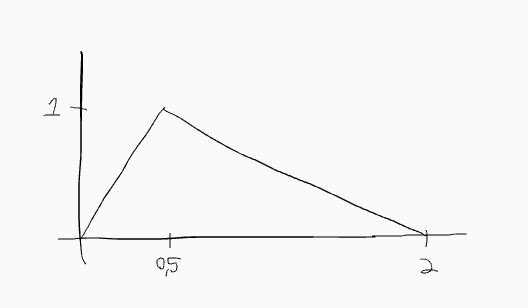
\includegraphics[scale=0.7]{q2}
\end{figure}

$f(x)\geq0$ Sim.\\

$\displaystyle\int_{0}^{\frac{1}{2}}2xdx+\int_{\frac{1}{2}}^{2}-\dfrac{2}{3}x+\dfrac{4}{3}dx=1$\qquad\qquad
$x^{2}\biggr|^{\frac{1}{2}}_{0}+\left(-\dfrac{x^{2}}{3}+\dfrac{4x}{3}\right)\biggr|^{2}_{\frac{1}{2}}=1$\\\\

$\left(\dfrac{1}{4}-0\right)+\left(\dfrac{4}{3}-\dfrac{7}{12}\right)=1$\qquad\qquad
$\dfrac{1}{4}+\dfrac{3}{4}=1$\qquad\qquad
$1=1$\\\\

$S_{X} = [0,2]$\\

\noindent b)\\

$F_{X}(x)$ para $\left[0,\dfrac{1}{2}\right]=\displaystyle\int_{0}^{x}2tdt$\qquad\qquad
$t^{2}\biggr|^{x}_{0}$\qquad\qquad
$x^2$\\\\

$F_{X}(x)$ para $\left[\dfrac{1}{2},2\right]=\displaystyle\int_{\frac{1}{2}}^{x}-\dfrac{2}{3}t+\dfrac{4}{3}dt$\qquad\qquad
$\displaystyle\dfrac{1}{3}\int_{\frac{1}{2}}^{x}-2t+4dt$\qquad\qquad
$\dfrac{1}{3}\left(-t^{2}+4t\right)\biggr|^{x}_{\frac{1}{2}}$\\\\

$\dfrac{1}{3}(-x^{2}+4x-1)$\\\\

$F_{X}(x)=\left\{\begin{array}{@{}l@{}}
	x^2\text{,\qquad\qquad\qquad se }\leq x<\leq\frac{1}{2},\\\\
	\dfrac{1}{3}(-x^{2}+4x-1)\text{, se }\frac{1}{2}\leq x\leq2,\\\\
	0\text{,\qquad\qquad\qquad\quad caso contrário.}
\end{array}\right.$

\begin{figure}[h!]
	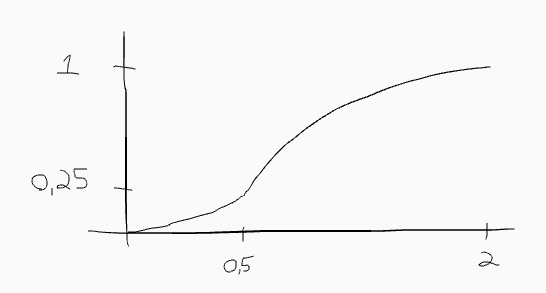
\includegraphics[scale=0.7]{q2b}
\end{figure}
	
\noindent c)\\

$P(0<x<1)=P\left( 0<x<\dfrac{1}{2}\right)+P\left(\dfrac{1}{2}<x<1\right)$\\\\

$\displaystyle\int_{0}^{\frac{1}{2}}2xdx+\int_{\frac{1}{2}}^{1}\dfrac{1}{3}(-2x+4)dx$\qquad\qquad
$x^{2}\biggr|^{\frac{1}{2}}_{0}+\dfrac{1}{3}(-x^2+4x)\biggr|^{1}_{\frac{1}{2}}$\qquad\qquad
$\left(\dfrac{1}{4}-0\right)+\dfrac{1}{3}\left(3-\dfrac{7}{4}\right)$\\\\

$\dfrac{1}{4}+\dfrac{1}{3}\cdot\dfrac{5}{4}$\qquad\qquad
$\dfrac{3}{12}+\dfrac{5}{12}$\qquad\qquad
$\dfrac{8}{12}$\qquad\qquad
$\dfrac{3}{4}$\\

	
	
	
	
	
	
	
	
	
	
	
\end{document}